\documentclass[10pt, a4paper]{article}
\usepackage[utf8]{inputenc}
\usepackage[frenchb]{babel}
\usepackage[OT1]{fontenc}
\usepackage{amsfonts, amsmath, amssymb, amsthm, dsfont, amsthm}
\usepackage{a4wide}
\usepackage[dvipsnames]{xcolor}
\usepackage{tikz} 
\usetikzlibrary{arrows,positioning,shapes}

\title{\textbf{Lab Report} \\ Week of 12/01/2016}
%\author{Olivier \textsc{Mangin}}
%\date{\today}

\definecolor{main}{named}{BurntOrange}
\definecolor{second}{named}{RoyalBlue}
%\newcommand{\maincolor}{orange}
%\newcommand{\secondcolor}{orange!20}
\newcommand{\strong}[1]{\textcolor{main}{\textbf{#1}}}
\newcommand{\stronger}[1]{\textcolor{second}{\textbf{#1}}}
\newcommand{\colored}[1]{\textcolor{main}{#1}}

% Affichage du titre avec les numéro et date de la semaine
\newcommand{\titre}[2]{
\noindent
\hspace{-10pt}
\begin{tabular}{lr}
  \hspace{0.58\textwidth} & \hspace{0.4\textwidth} \\
  \strong{\huge Lab Report} & \textbf{\Large #1} \medskip \\
  \textbf{\Large Name \& Roll} & {\large #2} ~\\
\end{tabular}

\vspace{20pt}
}

% Encadré ``En bref'' réumant les avancées et problèmes de la semaine
\newenvironment{enbref}{
\noindent\fcolorbox{main}{main}{
\begin{minipage}{\textwidth}
\textcolor{white}{\textbf{\large }}
\end{minipage}
} \\

}{
\begin{center}
  \strong{ \rule[2mm]{\textwidth}{3pt} }
\end{center}
\vspace*{-20pt}
}

% Affichage d'un titre de rubrique
\newcommand{\rubrique}[1]{
  \bigskip
  \begin{center}
  \begin{minipage}{\textwidth}
    \noindent\strong{{\large #1} \\
      \rule[2mm]{\textwidth}{1pt} }
  \end{minipage}
  \end{center}
  \vspace*{-20pt}
}

% Symbole utilisé en début de ligne des éléments
\newcommand{\doublerect}{
\begin{tikzpicture}
  \fill[color=main] (0,0) rectangle (4pt,-4pt);
  \fill[color=second] (2pt,-2pt) rectangle (6pt,-6pt);
\end{tikzpicture}
}

% Affichage d'un titre d'élément
\newcommand{\element}[1]{
  \medskip
  \noindent\textcolor{second}{ \doublerect \textbf{#1}}
}

% Pour les lectures, petit raccourci pour mettre en avant le niveau
% de lecture d'un article.
\newcommand{\lu}{\strong{[Lu]} }
\newcommand{\parcouru}{\strong{[Parcouru]} }
\newcommand{\alire}{\strong{[A lire]} }
\newcommand{\presentation}{\strong{[Présentation]} }
\newcommand{\keynote}{\strong{[Keynote]} }



\usepackage[pdfauthor={Name}, pdftitle={Weekly}, pdfsubject={Week 1}, pdfkeywords={},colorlinks=true,urlcolor=black,linkcolor=black, citecolor=black]{hyperref}
\usepackage{listings}
\usepackage{subfig}
\usepackage{graphicx}
\lstset{%
language=Matlab,
frame=single,
%numbers=left,
%numberstyle=\footnotesize,
%tabsize=2,
keepspaces=true,
columns=fullflexible,
basicstyle=\ttfamily\scriptsize,
keywordstyle=\color{blue}
}


\begin{document}

\renewcommand{\labelitemi}{\textcolor{main}{\small $\blacktriangleright$}}
\renewcommand{\labelitemii}{\textcolor{second}{\scriptsize \textbullet}}

\titre{Week 9}{03/04/2017}

\begin{enbref}
\element{Title}
\begin{itemize}
\item Implement Hidden Surface removal for a CUBE.\\
    1). OpenGL\\
\end{itemize}
\medskip
\end{enbref}

\rubrique{Procedure}
\vspace{0.5mm} \flushleft

\element {OpenGL}

\vspace{0.5mm} \flushleft
1). Choose N vertices of a CUBE and a viewing vector, then apply the algorithm  described below :
\begin{itemize}
\item Create a C file and name it as \textit{hsr.c}.
\item Following is the final code :
\begin{lstlisting}
#include "GL/glut.h"
#include "GL/gl.h"
#include <math.h>
#include <stdio.h>

int side = 0; int flag = 0;
float vx,vy,vz; int count =0; float a[2][3];
int calculate()
{
	float cross_product[3];
	cross_product[0] = a[0][1]*a[1][2] - a[0][2]*a[1][1];
	cross_product[1] = a[0][2]*a[1][0] - a[0][0]*a[1][2];
	cross_product[2] = a[0][0]*a[1][1] - a[0][1]*a[1][0];

	int dot_product = vx * cross_product[0] + vy * cross_product[1] + vz * cross_product[2];
	if(dot_product > 0)
	{
		printf("Cube's Face number  : %d is visible\n", count);
		return 1;
	}
	return 0;
}
void display_function_after()
{
	printf("\n************** Simulation Started **************\n\n");
	glClearColor(1.0, 1.0, 1.0, 1.0);
	glClear(GL_COLOR_BUFFER_BIT);
	glMatrixMode(GL_MODELVIEW);
    	glTranslatef(0.0, 0.0, -1.0);
    	glRotatef(-45, 0.0, 1.0, 0.0);
    	glRotatef(-45, 0.0, 0.0, 1.0);
	int vertices[6][4][3] =
	{
		{ {side , 0 , 0} , {side , side , 0} , {side , side , side} , {side , 0 , side} },
		{ {side , side , 0}, {0, side , 0} , {0 , side , side} , {side , side , side} },
		{ {0 , side , 0}  , {0 , side , side}, {0 , 0 , side},{0 , 0 , 0} },
		{ {0, 0, side}, {0 , 0 , 0}, {side, 0, 0}, {side , 0, side} },
		{ {side , 0, side } , {side , side , side} , {0, side, side} , {side, 0, side}},
		{ {side , 0 , 0} , {0, 0, 0} , {0, side, 0} , {side, side, 0}}
	};
	int i= 0 ; int j = 0 ;
	for(i = 0 ; i < 6 ; i++)
	{
		count = i+1;
		for(j = 0 ; j < 3 ; j++)
		{
			a[0][j] = vertices[i][3][j] - vertices[i][0][j];
            		a[1][j] = vertices[i][0][j] - vertices[i][1][j];
		}
		if(calculate())
		{
			glBegin(GL_QUADS);
			if(flag == 0) glColor3f(1.0, 0.1, 0.9);
			else if(flag == 1) glColor3f(0.5, 0.5, 0.5);
			else if(flag == 2) glColor3f(0.8, 0.4, 0.6);
			else if(flag == 3) glColor3f(1.0, 0.3, 1.0);
			else if(flag == 4) glColor3f(0.1, 0.9, 0.2);
			else 		   glColor3f(0.2, 0.9, 0.7);

			printf("The co-ordinates of visible surface are : \n\n");
			printf("x\ty\tz\n");
			printf("-----------------\n");
			printf("%d\t%d\t%d\n",vertices[i][0][0],vertices[i][0][1],vertices[i][0][2]);
			printf("%d\t%d\t%d\n",vertices[i][1][0],vertices[i][1][1],vertices[i][1][2]);
			printf("%d\t%d\t%d\n",vertices[i][2][0],vertices[i][2][1],vertices[i][2][2]);
			printf("%d\t%d\t%d\n",vertices[i][3][0],vertices[i][3][1],vertices[i][3][2]);
			printf("\n");
			glVertex3f(vertices[i][0][0]/10.0f, vertices[i][0][1]/10.0f, vertices[i][0][2]/10.0f);
            		glVertex3f(vertices[i][1][0]/10.0f, vertices[i][1][1]/10.0f, vertices[i][1][2]/10.0f);
            		glVertex3f(vertices[i][2][0]/10.0f, vertices[i][2][1]/10.0f, vertices[i][2][2]/10.0f);
            		glVertex3f(vertices[i][3][0]/10.0f, vertices[i][3][1]/10.0f, vertices[i][3][2]/10.0f);
            		flag++;
            		glEnd();
		}
	}
	printf(">> Only %d faces were visible\n",flag);
	printf("**************  Simulation Ended  **************\n");
	glFlush();
	glutSwapBuffers();
}
void display_function_Before()
{
	glClearColor(1.0, 1.0, 1.0, 1.0);
	glClear(GL_COLOR_BUFFER_BIT);
	glMatrixMode(GL_MODELVIEW);
    	glTranslatef(0.0, 0.0, -1.0);
	glRotatef(-45, 0.0, 1.0, 0.0);
    	glRotatef(-45, 0.0, 0.0, 1.0);
	int vertices[6][4][3] =
	{
		{ {side , 0 , 0} , {side , side , 0} , {side , side , side} , {side , 0 , side} },
		{ {side , side , 0}, {0, side , 0} , {0 , side , side} , {side , side , side} },
		{ {0 , side , 0}  , {0 , side , side}, {0 , 0 , side},{0 , 0 , 0} },
		{ {0, 0, side}, {0 , 0 , 0}, {side, 0, 0}, {side , 0, side} },
		{ {side , 0, side } , {side , side , side} , {0, side, side} , {side, 0, side}},
		{ {side , 0 , 0} , {0, 0, 0} , {0, side, 0} , {side, side, 0}}
	};
	int i = 0 ; int flag=0;
	for(i = 0 ; i < 6 ; i++)
	{
		glBegin(GL_QUADS);
		if(flag == 0) glColor3f(1.0, 0.1, 0.9);
		else if(flag == 1) glColor3f(0.5, 0.5, 0.5);
		else if(flag == 2) glColor3f(0.8, 0.4, 0.6);
		else if(flag == 3) glColor3f(1.0, 0.3, 1.0);
		else if(flag == 4) glColor3f(0.1, 0.9, 0.2);
		else 		   glColor3f(0.2, 0.9, 0.7);
		glVertex3f(vertices[i][0][0]/10.0f, vertices[i][0][1]/10.0f, vertices[i][0][2]/10.0f);
		glVertex3f(vertices[i][1][0]/10.0f, vertices[i][1][1]/10.0f, vertices[i][1][2]/10.0f);
		glVertex3f(vertices[i][2][0]/10.0f, vertices[i][2][1]/10.0f, vertices[i][2][2]/10.0f);
		glVertex3f(vertices[i][3][0]/10.0f, vertices[i][3][1]/10.0f, vertices[i][3][2]/10.0f);
		flag++;
		glEnd();
	}
	glFlush();
}
int main(int argc, char *argv[])
{
	printf("********  Provide the neccesary input  *********\n\n");
	printf("Enter the edge Length of the cube : "); scanf("%d",&side);
	printf("Enter the viewing vector : "); 		scanf("%f%f%f",&vx,&vy,&vz);
	glutInit(&argc,argv);
    	glutInitDisplayMode(GLUT_RGB);
    	glutInitWindowSize(400, 400);
    	gluOrtho2D(-200, 200, -200, 200);
	glutCreateWindow("Cube Before  : HSR");
	glutDisplayFunc(display_function_Before);
	glutCreateWindow("Cube After  : HSR");
	glutDisplayFunc(display_function_after);
	glutMainLoop();
	return 0;
}


\end{lstlisting}

\vspace{0.5mm}

\item Compile and run the executable file in terminal by typing in the following commands : \\

\vspace{0.5mm} \flushleft

\textit{(a)\hspace{2mm} gcc hsr.c -lGL -lGLU -lglut -ll -o hsr} \\
\textit{(b)\hspace{2mm} ./hsr}
\vspace*{1\baselineskip}
\end{itemize}

\rubrique{Output}
\begin{figure}[ht!]
\centering
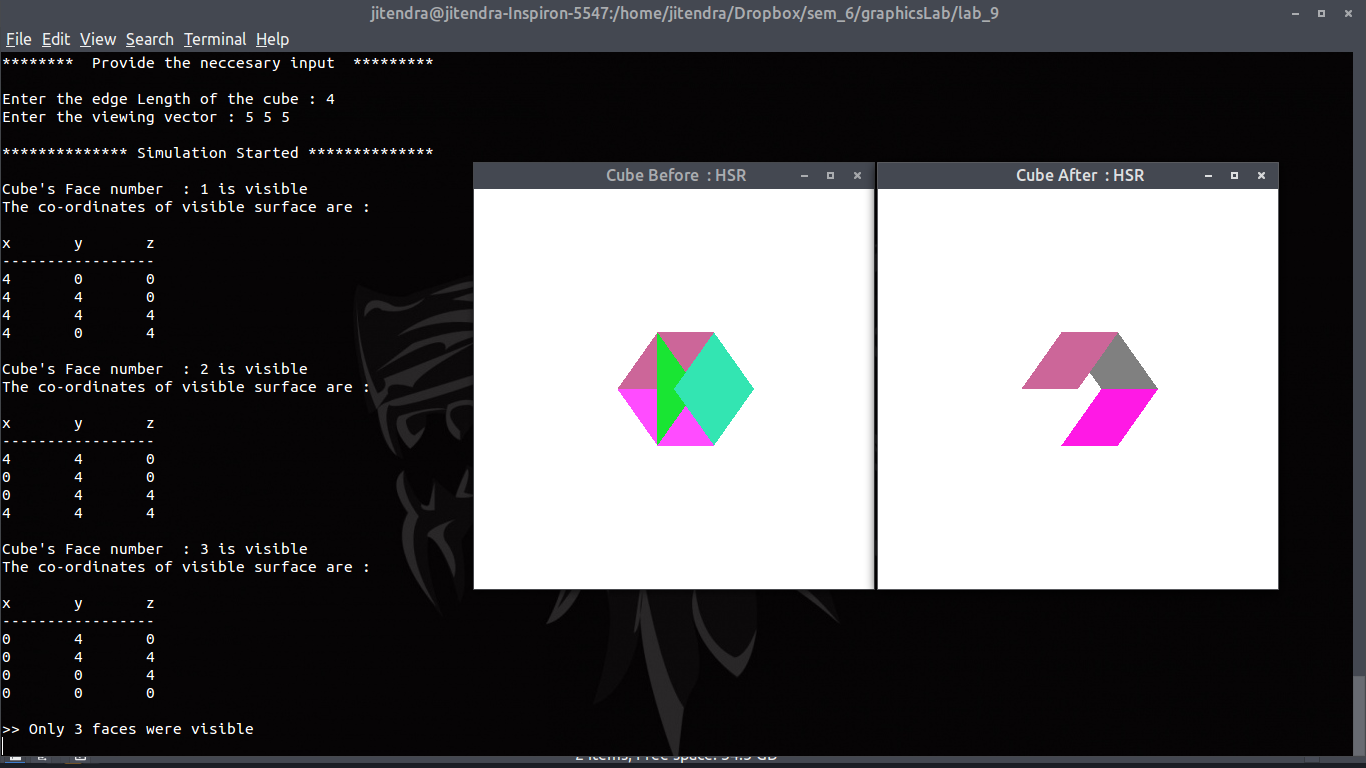
\includegraphics[width=150mm, height=100mm]{output1.png}
\caption{openGL output \label{overflow}}
\end{figure}
\begin{figure}[ht!]
\centering
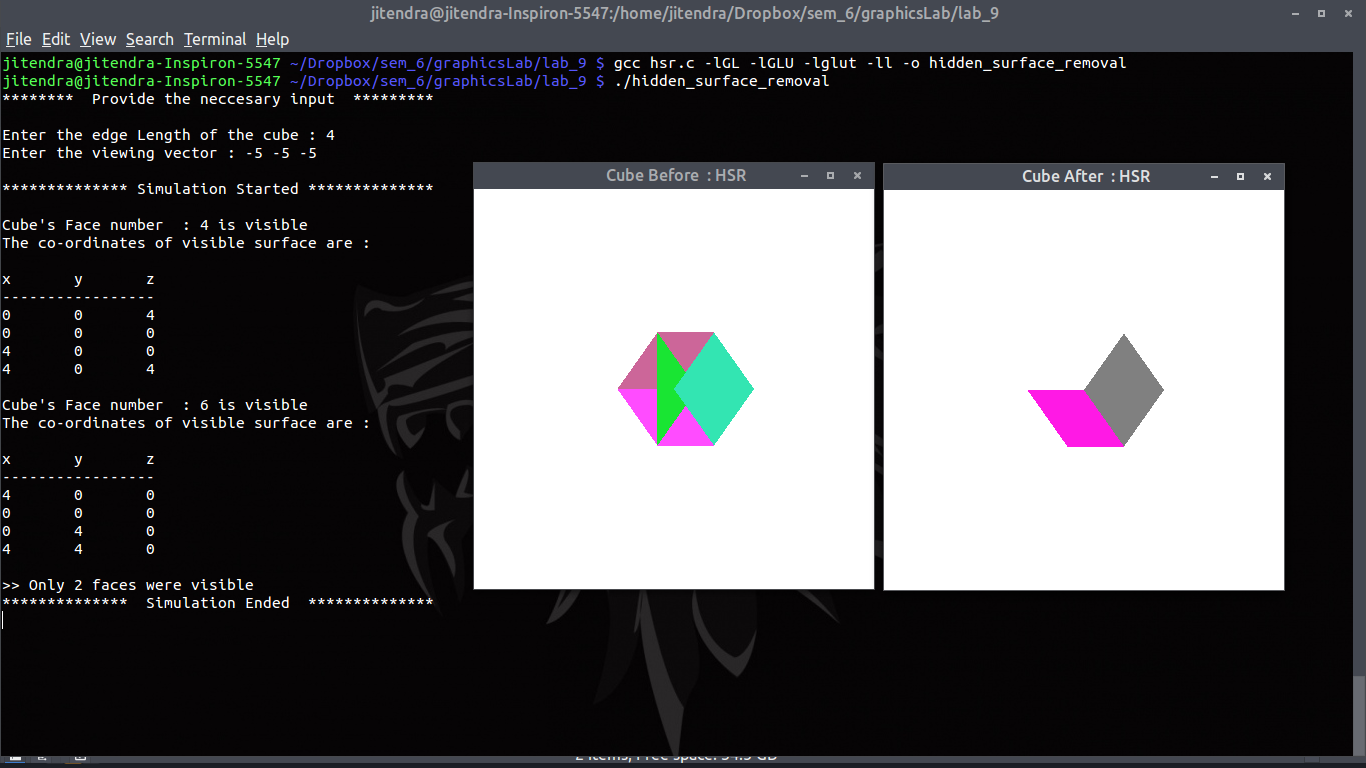
\includegraphics[width=150mm, height=100mm]{output2.png}
\caption{openGL output \label{overflow}}
\end{figure}
\end{document}
